%
% teil2.tex -- Beispiel-File für teil2
%
% (c) 2020 Prof Dr Andreas Müller, Hochschule Rapperswil
%

\section{Algorithmen}
\rhead{Algorithmen}

In diesem Abschnitt werden mehrere Algorithmen zur Berechnung der Matrizenmultiplikation vorgestellt, auch werden Bibliotheken zur unkomplizierten Verwendung von vordefinierten Algorithmen gezeigt.

\subsection{Standardalgorithmus}

Die Standardmethode ist im Algorithmus \ref{multiplikation:alg:smm} implementiert.
Hierf\"ur wurde die Gleichung \eqref{multiplikation:eq:MM} direkt umgesetzt.
Die \texttt{for i} Schleife iteriert \"uber alle Zeilen der $\mathbf{A}$ Matrix, die \texttt{for j} Schleife iteriert \"uber alle Spalten der $\mathbf{B}$ Matrix und die \texttt{for k} Schleife iteriert \"uber alle Eintr\"age dieser Zeilen bzw. Spalten.
\begin{algorithm}\footnotesize\caption{Matrizenmultiplikation}
	\label{multiplikation:alg:smm}
	\setlength{\lineskip}{7pt}
	\begin{algorithmic}[1]
		\Function{MM}{$\textbf{A}, \textbf{B}$}
		\State $sum \gets 0$
		\State $n \gets columns(\textbf{A}) == rows(\textbf{B})$
		\State $m \gets rows(\textbf{A})$
		\State $p \gets columns(\textbf{B})$
		\State $\textbf{C} \gets zeros(m,p)$
		\For{$i = 0,1,2 \dots,m-1$}
		\For{$j = 0,1,2 \dots,p-1$}
		\State $sum \gets 0$
		\For{$k = 0,1,2 \dots,n-1$}
		\State $sum \gets  sum + \textbf{A}[i][k] \cdot \textbf{B}[k][j]$
		\EndFor
		\State $\textbf{C}[i][j] \gets  sum $
		\EndFor
		\EndFor
		\State \textbf{return} $\textbf{C}$
		\EndFunction
	\end{algorithmic}
\end{algorithm}
Die Laufzeit dieser Struktur mit drei \texttt{for} Schleifen ist $\mathcal{O} (n^3)$.

\subsubsection{Divide and Conquer Methode}

F\"ur gewisse Algorithmen f\"uhren \textit{Divide and Conquer}  Ans\"atze \cite{multiplikation:DAC} zu markant besseren Laufzeiten.
Die Grundidee ist, dass ein Problem in mehrere, meist simplere und kleinere Teilprobleme aufgeteilt wird.
Das bekannteste Beispiel ist wohl die \textit{Fast Fourier Transform} wobei die Laufzeit von $\mathcal{O} (n^2)$ zu $\mathcal{O}(n \log n)$ verbessert werden kann.

Die Matrizenmultiplikation kann ebenfalls mit solch einem Ansatz berechnet werden.
Zur vereinfachten Veranschaulichung kann die Situation mit $\mathbf{A}$ und $\mathbf{B}$ der Gr\"osse $2^n \times 2^n$ verwendet werden.
Die Matrizen $\mathbf{A}$ und $\mathbf{B}$ werden in jeweils vier Blockmatrizen der Gr\"osse $2^{n-1} \times 2^{n-1}$ aufgeteilt.
Das Matrizenprodukt
\begin{equation}
\mathbf{A}\mathbf{B}=
\begin{bmatrix}
\mathbf{A}_{11} & \mathbf{A}_{12}\\
\mathbf{A}_{21} & \mathbf{A}_{22}
\end{bmatrix}
\begin{bmatrix}
\mathbf{B}_{11} & \mathbf{B}_{12}\\
\mathbf{B}_{21} & \mathbf{B}_{22}
\end{bmatrix}
=
\begin{bmatrix}
\mathbf{C}_{11} & \mathbf{C}_{12}\\
\mathbf{C}_{21} & \mathbf{C}_{22}
\end{bmatrix}
\end{equation}
mit \begin{equation}
\mathbf{C}_{ij} = \sum_{k=1}^{2n} \mathbf{A}_{ik} \mathbf{B}_{kj},
\label{multiplikation:eq:MM_block}
\end{equation}
ist identisch zu der Gleichung \eqref{multiplikation:eq:MM}, f\"ur die Multiplikation der Untermatrizen $\mathbf{A}_{ik}$ und $\mathbf{B}_{kj}$ wird die Matrizenmultiplikation verwendet.

Der Algorithmus \ref{multiplikation:alg:devide_mm} zeigt den \textit{Divide and Conquer} Ansatz,
Die Grundstruktur dieser Methode besteht aus dem rekursiven Aufruf der Funktion mit den erzeugten Blockmatrizen.
Der rekursive Aufruf wird bis zu der Gr\"osse der Matrizen von $N = 2 \times 2$ durchgef\"uhrt.
\begin{algorithm}\footnotesize\caption{Divide and Conquer Matrizenmultiplikation}
	\setlength{\lineskip}{7pt}
	\label{multiplikation:alg:devide_mm}
	\begin{algorithmic}
		\Function{MM}{$\textbf{A}, \textbf{B}, n$}
		\If{$n = 2$}
		\State  $ \mathbf{C} \gets zeros(n, n)$
		\State  $C[0, 0] \gets  A[0][0]\cdot B[0][0]+A[0][1]\cdot B[1][0]$
		\State  $C[0, 1] \gets  A[0][0]\cdot B[0][1]+A[0][1]\cdot B[1][1]$
		\State  $C[1, 0] \gets  A[1][0]\cdot B[0][0]+A[1][1]\cdot B[1][0]$
		\State  $C[1, 1] \gets  A[1][0]\cdot B[0][1]+A[1][1]\cdot B[1][1]$
		\Else
		\State  $ m \gets n/2$
		\State $\mathbf{A11}, \mathbf{A12}, \mathbf{A21}, \mathbf{A22} \gets \mathbf{A}[:m][:m], \mathbf{A}[:m][m:], \mathbf{A}[m:][:m], \mathbf{A}[m:][m:]$
		\State $\mathbf{B11}, \mathbf{B12}, \mathbf{B21}, \mathbf{B22} \gets \mathbf{B}[:m][:m], \mathbf{B}[:m][m:], \mathbf{B}[m:][:m], \mathbf{B}[m:][m:]$

		\State $\mathbf{C11} \gets \text{MM}(\mathbf{A11}, \mathbf{B11},n) + \text{MM}(\mathbf{A12}, \mathbf{B21},n)$
		\State $\mathbf{C12} \gets \text{MM}(\mathbf{A11},\mathbf{B12},n) + \text{MM}(\mathbf{A12}, \mathbf{B22},n)$
		\State $\mathbf{C21} \gets \text{MM}(\mathbf{A21}, \mathbf{B11},n) + \text{MM}(\mathbf{A22}, \mathbf{B21},n)$
		\State $\mathbf{C22} \gets \text{MM}(\mathbf{A21}, \mathbf{B12},n) + \text{MM}(\mathbf{A22}, \mathbf{B22},n)$
		\State $  C \gets vstack(hstack(C11, C12), hstack(C21, C22))$

		\EndIf
		\State \textbf{return} $\textbf{C}$

		\EndFunction
	\end{algorithmic}
\end{algorithm}

Die Laufzeit dieser rekursiven Funktion kann mit dem \textit{Master Theorem} \cite{multiplikation:master_theorem} berechnet werden. Das \textit{Master Theorem} bestimmt die Zeitkomplexit\"at von rekursiven Algorithmen.
Ohne auf dieses vertieft einzugehen, bestimmt die Anzahl rekursiver Aufrufe $\mathcal{T} $ der Funktion die Laufzeit.
In diesem Fall wird die Funktion pro Durchlauf acht mal rekursiv aufgerufen, dies f\"uhrt zu
\begin{equation} \label{multiplikation:eq:laufzeitdac}
	\mathcal{T}(n) =	8 \cdot \mathcal{T} \left(\frac{n}{2}\right ) + n^2  = \mathcal{O}(n^{\log_2 8}) = \mathcal{O}  (n^{3} ),
\end{equation}
also einer kubischen Laufzeit.
Die Addition zweier Matrizen $\mathbf{A} + \mathbf{B} = \mathbf{C}$ hat eine Laufzeit von $\mathcal{O}(n^{2})$ und kann neben dem dominierendem Anteil von $\mathcal{O}(n^{3})$ ignoriert werden.
In diesem Fall hat der \textit{Divide and Conquer} Ansatz zu keiner Verbesserung gef\"uhrt.


\subsection{Strassens Algorithmus}

Strassens Algorithmus \cite{multiplikation:strassen_1969} beschreibt die Matrizenmultiplikation mit einer Vielzahl von Additionen, Subtraktionen und Multiplikationen von Blockmatrizen.
Die sieben grundlegenden Terme
\begin{equation} \label{multiplikation:eq:strassen}
\begin{split}
\text{\textbf{P}}   &= \left(\mathbf{A}_{11} + \mathbf{A}_{22}\right ) \cdot \left(\mathbf{B}_{11} + \mathbf{B}_{22}\right ) \\
\text{\textbf{Q}}  &= \left(\mathbf{A}_{21} + \mathbf{A}_{22}\right ) \cdot \mathbf{B}_{11} \\
\text{\textbf{R}} &= \mathbf{A}_{11} \cdot \left(\mathbf{B}_{12}-\mathbf{B}_{22}\right ) \\
\text{\textbf{S}}  &= \mathbf{A}_{22} \cdot \left(-\mathbf{B}_{11}+\mathbf{B}_{21}\right ) \\
\text{\textbf{T}}   &= \left(\mathbf{A}_{11} + \mathbf{A}_{12}\right ) \cdot \mathbf{B}_{22} \\
\text{\textbf{U}}  &= \left(-\mathbf{A}_{11} + \mathbf{A}_{21}\right ) \cdot \left(\mathbf{B}_{11} + \mathbf{B}_{12}\right ) \\
\text{\textbf{V}} &= \left(\mathbf{A}_{12} - \mathbf{A}_{22}\right ) \cdot \left(\mathbf{B}_{21} + \mathbf{B}_{22}\right )
\end{split}
\end{equation}
aus $\mathbf{A}$ und $\mathbf{B}$ werden f\"ur die Berechnung der Bl\"ocke
\begin{equation} \label{multiplikation:eq:strassen2}
\begin{split}
\mathbf{C}_{11} &= \text{\textbf{P}} + \text{\textbf{S}} - \text{\textbf{T}} + \text{\textbf{V}} \\
\mathbf{C}_{21} &= \text{\textbf{R}} + \text{\textbf{T}} \\
\mathbf{C}_{12} &= \text{\textbf{Q}} + \text{\textbf{S}}\\
\mathbf{C}_{22} &= \text{\textbf{P}} + \text{\textbf{R}} - \text{\textbf{Q}} + \text{\textbf{U}}
\end{split}
\end{equation}
der Matrix $\mathbf{C}$ gebraucht.
\begin{algorithm}\footnotesize\caption{Strassen Matrizenmultiplikation}
	\label{multiplikation:alg:strassen}
	\setlength{\lineskip}{7pt}
	\begin{algorithmic}
		\Function{strassen}{$\textbf{A}, \textbf{B}, n$}
		\If{$n = 2$}
		\State  $ \mathbf{C} \gets zeros((n, n))$
		\State $P  \gets (A[0][0]+A[1][1])\cdot( B[0][0]+B[1][1])$
		\State   $Q  \gets (A[1][0]+A[1][1])\cdot B[0][0]$
		\State   $R  \gets A[0][0]\cdot (B[0][1]-B[1][1])$
		\State   $S  \gets A[1][1]\cdot (B[1][0]-B[0][0])$
		\State   $T  \gets (A[0][0]+A[0][1])\cdot B[1][1]$
		\State   $U  \gets (A[1][0]-A[0][0])\cdot (B[0][0]+B[0][1])$
		\State   $V  \gets (A[0][1]-A[1][1])\cdot (B[1][0]+B[1][1])$
		\State   $C[0][0]  \gets P+S-T+V$
		\State   $C[0][1]  \gets R+T$
		\State   $C[1][0]  \gets Q+S$
		\State   $C[1][1]  \gets P+R-Q+U$
		\Else
		\State  $ m \gets n/2$
		\State $\mathbf{A11}, \mathbf{A12}, \mathbf{A21}, \mathbf{A22} \gets \mathbf{A}[:m][:m], \mathbf{A}[:m][m:], \mathbf{A}[m:][:m], \mathbf{A}[m:][m:]$
		\State $\mathbf{B11}, \mathbf{B12}, \mathbf{B21}, \mathbf{B22} \gets \mathbf{B}[:m][:m], \mathbf{B}[:m][m:], \mathbf{B}[m:][:m], \mathbf{B}[m:][m:]$

		\State $ \mathbf{P} \gets \text{strassen}((\mathbf{A11}+ \mathbf{A22}),(\mathbf{B11}+\mathbf{B22}), m)$
		\State $ \mathbf{Q} \gets \text{strassen}((\mathbf{A21}+ \mathbf{A22}), \mathbf{B11},m)$
		\State $ \mathbf{R} \gets \text{strassen}( \mathbf{A11},(\mathbf{B12}-  \mathbf{B22}),m)$
		\State $ \mathbf{S} \gets \text{strassen}( \mathbf{A22},(\mathbf{B21}-  \mathbf{B11}),m)$
		\State $ \mathbf{T} \gets \text{strassen}((\mathbf{A11}+ \mathbf{A12}), \mathbf{B22},m)$
		\State $ \mathbf{U} \gets \text{strassen}((\mathbf{A21}- \mathbf{A11}),(\mathbf{B11}+\mathbf{B12}),m)$
		\State $ \mathbf{V} \gets \text{strassen}((\mathbf{A12}- \mathbf{A22}),(\mathbf{B21}+\mathbf{B22}),m)$



		\State   $\mathbf{C11}  \gets \mathbf{P+S-T+V}$
		\State   $\mathbf{C12}  \gets \mathbf{R+T}$
		\State   $\mathbf{C21}  \gets \mathbf{Q+S}$
		\State   $\mathbf{C22}  \gets \mathbf{P+R-Q+U}$
		\State $  C \gets vstack(hstack(C11, C12), hstack(C21, C22))$

		\EndIf
		\State \textbf{return} $\textbf{C}$

		\EndFunction
	\end{algorithmic}
\end{algorithm}
Strassens Methode wird in der Abbildung \ref{multiplikation:fig:strassen} grafisch dargestellt.
Jedes Feld steht f\"ur eine Multiplikation zweier Matrizenelementen von $\mathbf{A}$ oder $\mathbf{B}$ .
Die gr\"unen Felder auf der linken Seite, zeigen die Addition, welche f\"ur den dazugeh\"origen Term ben\"otigt wird.
Die sieben Spalten beschreiben die Matrizen $\mathbf{P,Q,R, \ldots, V}$.
Rote Felder stehen f\"ur eine Subtraktion und die gr\"unen f\"ur eine Addition.
Graue Felder bedeuten, dass die dazugehörige Spalte nicht für die Berechnung benötigt wird.
\begin{figure}
	\center
	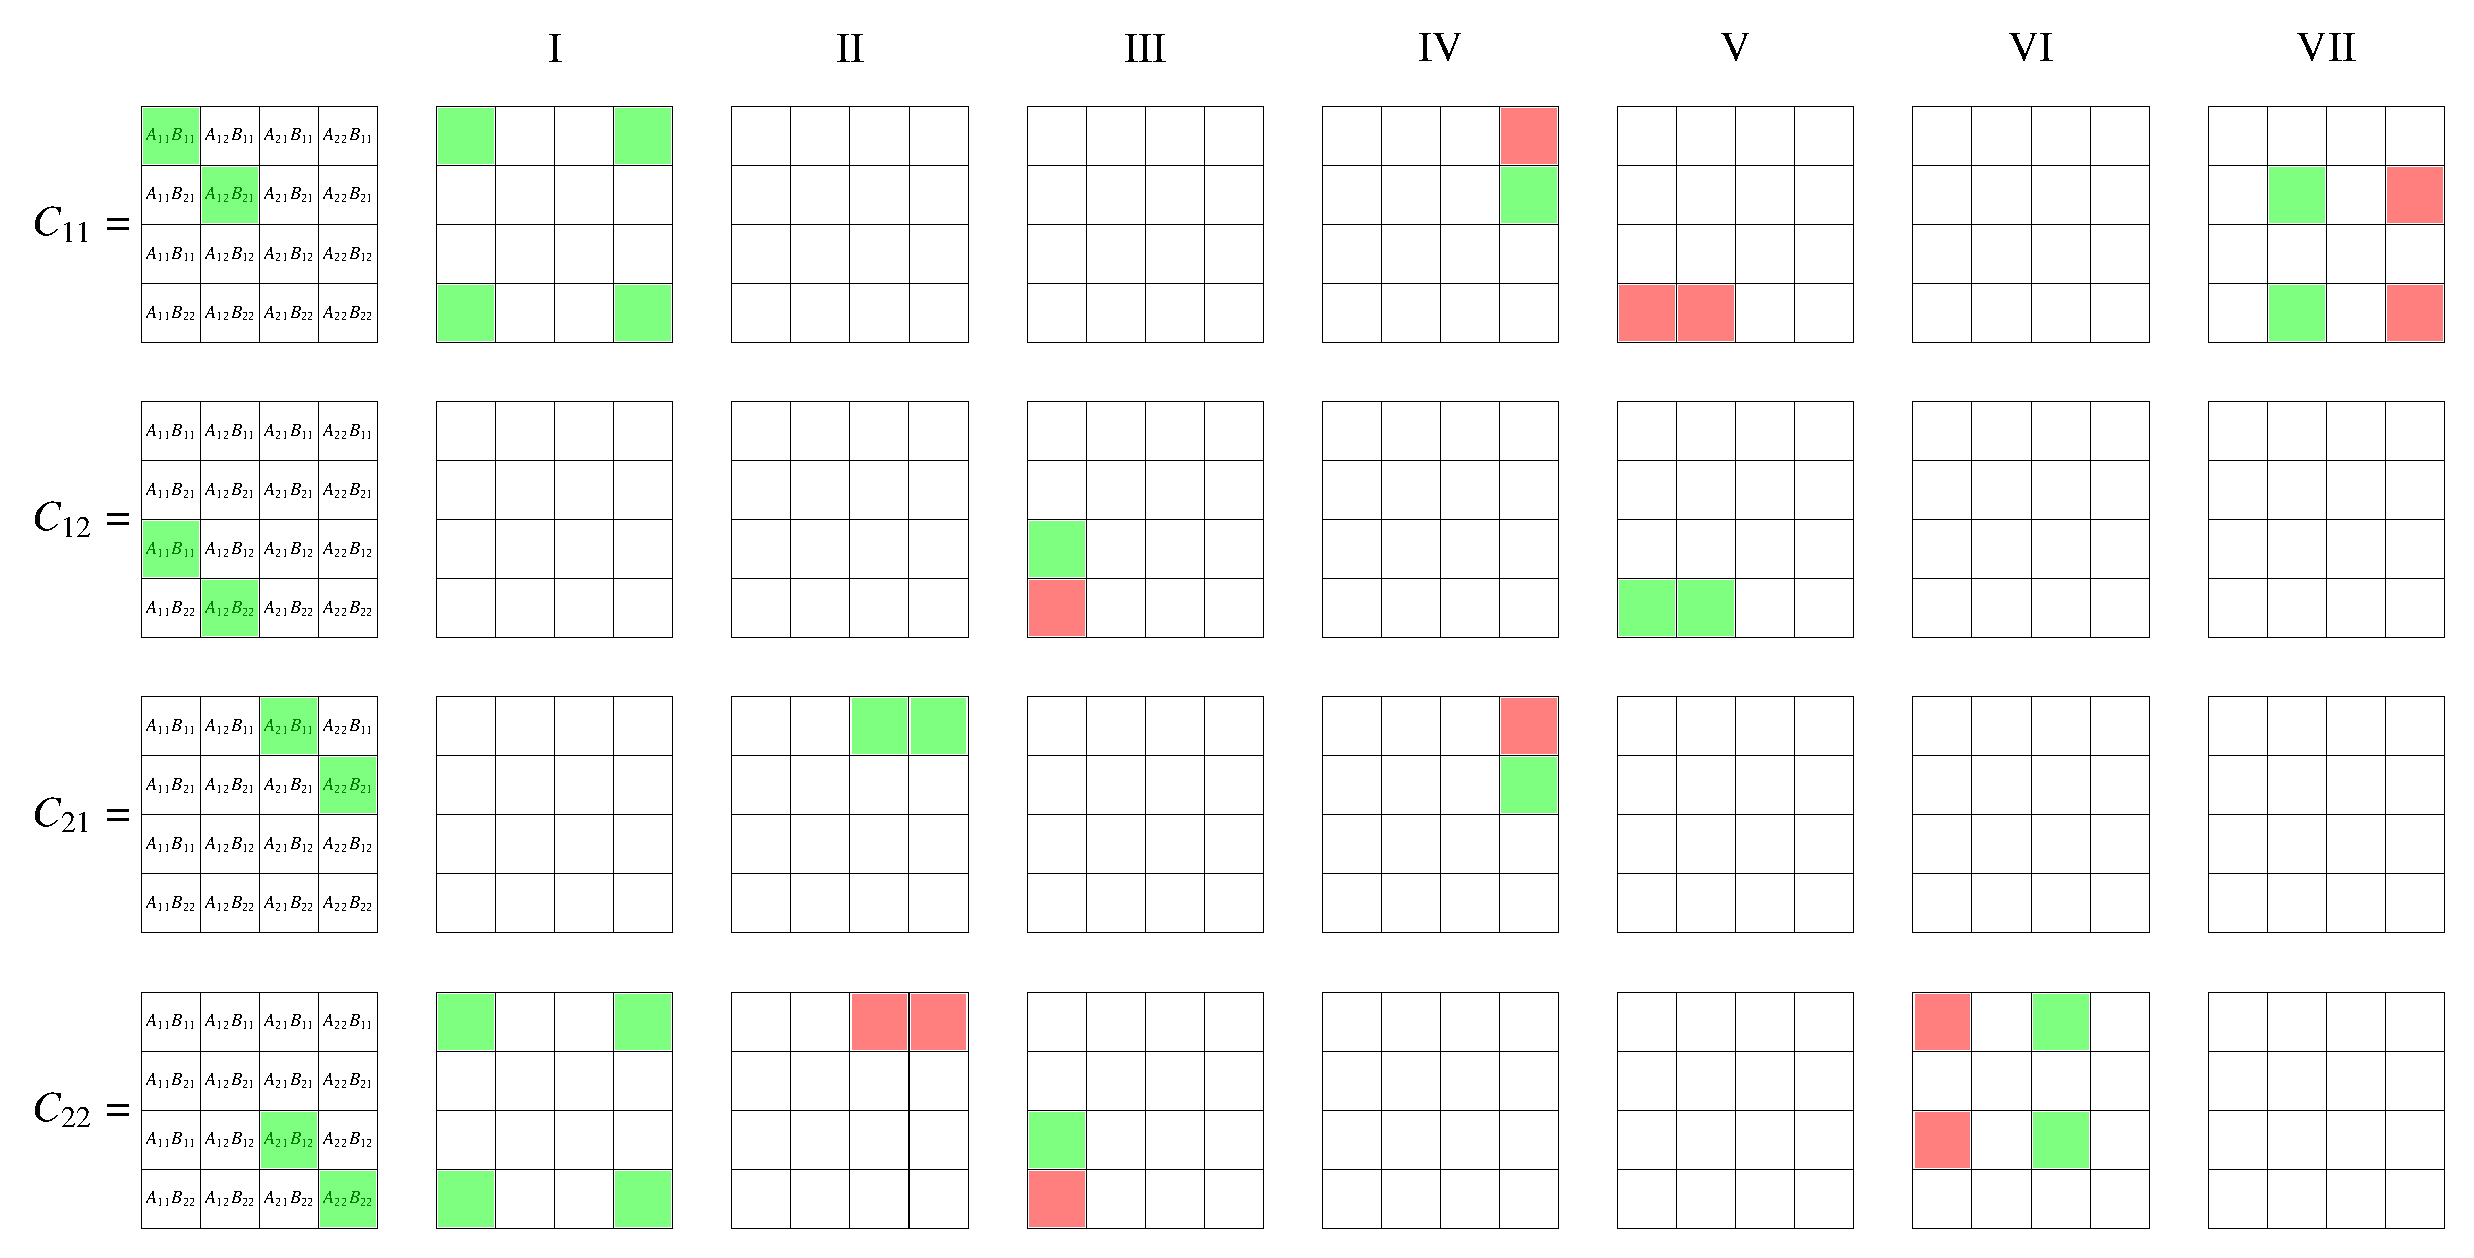
\includegraphics[width=\linewidth]{papers/multiplikation/images/strassen.pdf}
	\caption{Der Algorithmus von Strassen verwendet Multiplikationen zur Berechnung der sieben Blockmatrizen $\mathbf{P}$ bis $\mathbf{V}$ aus $\mathbf{A}$ und $\mathbf{B}$, aus denen sich die Blöcke es Produktes $\mathbf{C}=\mathbf{AB}$ ausschliesslich durch Addition und Subtraktion bilden lassen. Die einzelnen Felder in den Quadraten stellen alle möglichen Produkte von Matrizen $\mathbf{A}_{ik}$ und $\mathbf{B}_{jl}$ dar. In den grossen Quadraten am linken Rand sind diejenigen Produkte grün markiert, welche zusammen die entsprechenden Blöcke $\mathbf{C}_{il}$ von $\mathbf{C}$ ergeben. In den Spalten $\mathbf{P}$ bis $\mathbf{V}$ sind die Produkte farblich hervorgehoben, die in der Definition der entsprechenden Matrix vorkommen. Grün und rot symbolisieren die Vorzeichen, mit denen die Produkte kombiniert werden müssen. Graue Felder werden für die Berechnung von $\mathbf{C}_{il}$ nicht benötigt.}
	\label{multiplikation:fig:strassen}
\end{figure}

Die Funktion wird sieben mal rekursiv aufgerufen.
Dies f\"uhrt nach dem \textit{Master Theorem} zu einer Laufzeit von
\begin{equation} \label{multiplikation:eq:laufzeitstrassen}
\mathcal{T}(n) =
7 \cdot \mathcal{T}\left(\frac{n}{2}\right) + n^2  = \mathcal{O}(n^{\log_2 7} ) = \mathcal{O}(n^{2.8074}  )
\end{equation}
und ist somit schneller als die Standardmethode.
Man beachte, dass die Anzahl von Additionen und Subtraktionen gr\"osser und die Anzahl der Multiplikationen kleiner wurde.

\subsection{Winograds Algorithmus}

Einen weiteren Ansatz lieferte Shmuel Winograd im Jahre 1968 \cite{multiplikation:winograd_1968}.
Er beschrieb einen neuen Algorithmus f\"ur das Skalarprodukt
\begin{equation} \label{multiplikation:eq:skalar}
	\langle x,y \rangle = \sum_{i=1}^{n}x_i y_i.
\end{equation}
F\"ur jeden Vektor berechne
\begin{equation}
	\xi = \sum_{j=1}^{ \lfloor n/2 \rfloor} x_{2j-1} \cdot x_{2j}
\end{equation}
und
\begin{equation}
	\eta = \sum_{j=1}^{ \lfloor n/2 \rfloor} y_{2j-1} \cdot y_{2j},
\end{equation}
die jeweils nur von $x$ und $y$ abhängen.
Dazu werden $2 \cdot  \lfloor n/2 \rfloor \leq n$ Multiplikationen benötigt.
Das Skalarprodukt ist nun geben mit
\begin{equation}
	\langle x,y \rangle =
	\begin{cases}
	 \displaystyle \quad \sum_{j=1}^{ \lfloor n/2 \rfloor} (x_{2j-1} + y_{2j})(x_{2j}+y_{2j-1})-\xi - \eta & \text{wenn  $n$ gerade}\\
	\displaystyle  \quad \sum_{j=1}^{ \lfloor n/2 \rfloor} (x_{2j-1} + y_{2j})(x_{2j}+y_{2j-1})-\xi - \eta + x_n y_n & \text{wenn  $n$ ungerade}.
	\end{cases}
\end{equation}
Das Skalarprodukt kann also mit $ \lfloor \frac{n+1}{2} \rfloor$ weiteren Multiplikationen berechnet werden.
Angenommen man hat $N$ Vektoren, mit welchen man $T$ Skalarprodukte berechnen m\"ochte.
Daf\"ur werden $N\lfloor n/2 \rfloor + T\lfloor (n+1)/2 \rfloor $ Multiplikationen ben\"otigt.
Die Summen f\"ur $\xi$ und $\eta$ m\"ussen nur einmal berechnet werden.
Für die ursprüngliche Gleichung \eqref{multiplikation:eq:skalar} für das Skalarprodukt benötigt man $Tn$ Multiplikationen.
Damit können wir die Laufzeit der Methode von Winograd mit der Laufzeit der Standardmethode vergleichen. Sie ist kleiner als die Laufzeit für die Standardmethode, wenn gilt
\begin{equation}\label{multiplikation:eq:eff}
\begin{array}{crcl}
                & N\lfloor n/2\rfloor + T\lfloor(n+1)/2\rfloor \approx Nn/2 + Tn/2 & \le & Tn   \\
\Leftrightarrow &                                                             Nn/2 & \le & Tn/2 \\
\Leftrightarrow &                                                                N & \le & T.
\end{array}
\end{equation}
Eine Matrizenmultiplikation mit $\mathbf{A}$ einer $m \times n$ und $\mathbf{B}$ einer $n \times p$ Matrix, entspricht $N=m+p$ Vektoren mit welchen man $T=mp$ Skalarprodukte berechnet.
Dies f\"uhrt zu
\begin{equation}
		(m+p) \left \lfloor \frac{n}{2} \right \rfloor + mp \left \lfloor \frac{n+1}{2} \right \rfloor = \frac{mn}{2} + \frac{pn}{2} + \frac{mpn}{2} + \frac{mp}{2}
\end{equation}
Multiplikationen.
Wenn $m,p,n$ gross werden, dominiert der Term $\frac{mpn}{2}$ und es werden $\frac{mpn}{2}$ Multiplikationen ben\"otigt, was im Vergleich zu den $mpn$ Multiplikation der Standardmethode nur die H\"alfte ist.
Mit dem gleichen Ansatz wie in der Gleichung \eqref{multiplikation:eq:eff} aber mit quadratischen Matrizen, muss
\begin{align}
	\begin{split}
N=2n, &\quad T = n^2 \\
	2n &\leq n^2 \\
	2 &\leq n
\end{split}
\end{align}
sein, damit man etwas einspart.
Die Implementation kann Algorithmus \ref{multiplikation:alg:winograd} entnommen werden.
Falls $m=n=p$, werden $\frac{n^3}{2}$ Multiplikationen benötigt.
Im Abschnitt \ref{muliplikation:sec:bigo} wurde bereits erläutert: falls $n \rightarrow \infty$ können Konstanten vernachlässigt werden und
 somit entsteht für diesen Algorithmus wieder die ursprüngliche Laufzeit von $\mathcal{O}(n^3 )$.
\begin{algorithm}\footnotesize\caption{Winograds Matrizenmultiplikation}
	\setlength{\lineskip}{7pt}
	\label{multiplikation:alg:winograd}
	\begin{algorithmic}
		\Function{Winograd}{$\textbf{A}, \textbf{B}, n$}
		\State  $ m \gets rows(\mathbf{A})$
		\State  $ n \gets columns(\mathbf{A}) == rows(\mathbf{B})$
		\State  $ p \gets columns(\mathbf{B})$
		\State  $ \mathbf{\xi} \gets zeros(m)$
		\State  $ \mathbf{\eta} \gets zeros(p)$


		\For{$i = 0,1,2 \dots,m-1$}
		\For{$j = 0,1,2 \dots,\lfloor n/2 \rfloor-1$}
		\State $\xi[i] \gets \xi[i]+A[i,2 j]A[i,2 j+1]$
		\EndFor
		\EndFor

		\For{$i = 0,1,2 \dots,p-1$}
		\For{$j = 0,1,2 \dots,\lfloor n/2 \rfloor-1$}
		\State $\eta[i] \gets   \eta[i]+B[2 j,i]B[2 j+1,i]$
		\EndFor
		\EndFor

		\If{$n \% 2 == 0$}
		\For{$i = 0,1,2 \dots,m-1$}
		\For{$j = 0,1,2 \dots,p-1$}
		\State $ab \gets 0$
		\For{$k = 0,1,2 \dots,\lfloor n/2 \rfloor-1$}
		\State $ab \gets ab + (A[i,2k]+B[2k+1,j])(A[i,2k+1]+B[2k,j])$
		\EndFor
		\State $C[i,j] \gets ab-\eta[j]-\xi[i]$
		\EndFor
		\EndFor
    \Else
		\For{$i = 0,1,2 \dots,n-1$}
		\For{$j = 0,1,2 \dots,n-1$}
		\State $ab \gets 0$
		\For{$k = 0,1,2 \dots,\lfloor n/2 \rfloor-1$}
		\State $ab \gets ab + (A[i,2k]+B[2k+1,j])(A[i,2k+1]+B[2k,j])$
		\EndFor
		\State $C[i,j] \gets ab-\eta[j]-\xi[i]+A[i,-1]B[-1,j]$
		\EndFor
		\EndFor
		\EndIf
		\State \textbf{return} $\textbf{C}$

		\EndFunction
	\end{algorithmic}
\end{algorithm}


\subsection{Basic Linear Algebra Subprograms (BLAS)}

Die gebräuchliche Methode f\"ur die Anwendung einer optimierten Matrizenmultiplikation ist die Verwendung einer Subroutine aus den \textit{Basic Linear Algebra Subprograms (BLAS)}  \cite{multiplikation:BLAS}.
Die meisten numerischen Bibliotheken von high-level Skriptsprachen wie \texttt{Matlab}, \texttt{NumPy (Python)}, \texttt{GNU Octave} oder \texttt{Mathematica} ben\"utzen eine Form von \textit{BLAS}.

\textit{BLAS} sind dabei in drei unterschiedliche Levels aufgeteilt.

\begin{itemize}
	\item Level 1
	\begin{itemize}
		\item Operationen der Art: $\mathbf{y} \leftarrow \alpha \mathbf{x}+\mathbf{y}$
		\item Dieses Level hat $\mathcal{O}(n)$ Charakteristik
	\end{itemize}
	\item Level 2
	\begin{itemize}
		\item Operationen der Art: $\mathbf{y} \leftarrow \alpha \mathbf{A}\mathbf{x}+\beta  \mathbf{y}$
		\item Dieses Level hat $\mathcal{O}(n^2)$ Charakteristik
		\end{itemize}
		\item Level 3
		\begin{itemize}
			\item Operationen der Art: $\mathbf{C} \leftarrow \alpha \mathbf{A}\mathbf{B}+\beta\mathbf{C}$
			\item Dieses Level hat $\mathcal{O}(n^3)$ Charakteristik
			\end{itemize}
\end{itemize}

Die \textit{BLAS} sind auf die modernen Computerprozessoren optimiert und k\"onnen dank einer ausgeklügelter Verwendung der Speicherarchitektur zu erheblichen Leistungsoptimierungen f\"uhren.


%\subsubsection{General Matrix Multiplication (GEMM)}
%
%Die \textit{Double-GEMM} \cite{multiplikation:DGEMM} ist definiert als:
%
%\textit{DGEMM  performs one of the matrix-matrix operations}
%$$
% C := \alpha \cdot op( A )\cdot op( B ) + \beta \cdot C,
% $$
% \textit{where  op( X ) is one of}
%$$
%op( X ) = X  \quad \text{ or } \quad  op( X ) = X^T,
%$$
% \textit{alpha and beta are scalars, and A, B and C are matrices, with op( A )
% an m by k matrix,  op( B )  a  k by n matrix and  C an m by n matrix.
% }

%Die Implementation von $\alpha\mathbf{A}\mathbf{B} + \beta \mathbf{C} = \mathbf{C}$, wobei  $\alpha = 1.0$ und $\beta = 0.0$ in der \texttt{C}-Version von \textit{BLAS}, ist als
%\begin{lstlisting}[style=multiplikationC]
%cblas_dgemm(CblasRowMajor, CblasNoTrans, CblasNoTrans,
%      m, n, k, 1, A, m , B, k, 0, C, m);
%\end{lstlisting}
%definiert.



\section{Implementation}\label{multiplikation:section:Implementation}
\rhead{Implementation}

Folgende Algorithmen wurden jeweils in \texttt{C} und \texttt{Python} implementiert.
\begin{itemize}
	\item Standard Matrizenmultiplikation
	\item \textit{Divide and Conquer} Matrizenmultiplikation
	\item Strassens Matrizenmultiplikation
	\item Winograds Matrizenmultiplikation
	\item \texttt{BLAS} Matrizenmultiplikation in \texttt{C}
	\item \texttt{Numpy} Matrizenmultiplikation in \texttt{Python}
\end{itemize}

Der Code kann im zum Buch gehörigem \textit{GitHub} \footnote{\url{https://github.com/AndreasFMueller/SeminarMatrizen.git}} Repository gefunden werden.
Anzumerken ist, dass die Matrizenmultiplikation von \texttt{NumPy} als einzige Implementation Multiprocessing und Multithreading verwendet, dies f\"uhrt zu den tiefen Messzeiten.
In Abbildung \ref{multiplikation:fig:python} und Abbildung \ref{multiplikation:fig:c_meas_4096} sind de Messresultate grafisch dargestellt. Die selben Messresultate sind tabellarisch in Tabelle \ref{multiplikation:tab:messung_Python} und Tabelle \ref{multiplikation:tab:messung_C} ersichtlich.

Die gezeigten Algorithmen haben alle eine Laufzeit der Form $\mathcal{O}(n^k) $.
Bei einer doppelt logarithmischen Darstellung unterscheiden sich diese in Geraden mit unterschiedlichen Steigungen.
Bei den grafisch gezeigten Messresultate, können diese Steigungen gut erkannt werden, wobei die tiefere Laufzeit des Strassen Algorithmus eindrücklich zu sehen ist.
Der benötigte Overhead der Algorithmen zeigt sich in unterschiedlichen $y$-Achsenschnittpunkte.

In der Messung mit der Programmiersprache \texttt{C} kann ein typischer Cache-Effekt beobachtet wer-
den.
Bei den Algorithmen von Winograd und der Standardmethode hat bei einer Matrizengrösse von $n = 2048$ wohl eine Zeile der Matrix nicht an einer Cache Speicherstelle Platz.
Diese beiden Algorithmen sind die Einzigen, welche \texttt{for}-Schleifen über die ganze Breite der Matrizen verwenden.
Dies führt dazu, dass ganze Zeilen zwischengespeichert werden müssen.
Bei den anderen Algorithmen ist dies nicht der Fall.

Die Hardwareinformationen des verwendeten Computers sind in der Tabelle \ref{multiplikation:tab:pc_config} aufgelistet.


\begin{table}
			 \begin{center}
					 \begin{tabular}{r l l l l l}
							 \hline
							 \hline
							 \textbf{n} & \textbf{MM (\textit{s})} &  \textbf{MM DC (\textit{s})} & \textbf{Strassen (\textit{s})}  & \textbf{Winograd (\textit{s})} & \textbf{BLAS (\textit{s})} \\
							 \hline
							 \multicolumn{6}{c}{} \\
							 \textbf{32}   & \phantom{000}0.000089 & \phantom{000}0.000594 & \phantom{000}0.0005  & \phantom{0000}0.00008 & \phantom{00}0.000021  \\
							 \textbf{64}   & \phantom{000}0.00069  & \phantom{000}0.0044   & \phantom{000}0.0036  & \phantom{0000}0.00064 & \phantom{00}0.00018   \\
							 \textbf{128}  & \phantom{000}0.0057   & \phantom{000}0.035    & \phantom{000}0.025   & \phantom{0000}0.0052  & \phantom{00}0.0012    \\
							 \textbf{256}  & \phantom{000}0.052    & \phantom{000}0.29     & \phantom{000}0.178   & \phantom{0000}0.053   & \phantom{00}0.0096     \\
							 \textbf{512}  & \phantom{000}0.51     & \phantom{000}2.22     & \phantom{000}1.25    & \phantom{0000}0.55    & \phantom{00}0.077     \\
							 \textbf{1024} & \phantom{000}4.50     & \phantom{00}17.65     & \phantom{000}8.83    & \phantom{0000}4.67    & \phantom{00}0.764     \\
							 \textbf{2048} & \phantom{0}129.28     & \phantom{0}141.61     & \phantom{00}61.901   & \phantom{00}136.67    & \phantom{00}7.63      \\
							 \textbf{4096} & 1111.31               & 1147.10               & \phantom{0}414.64    & \phantom{0}1179.26    & \phantom{0}55.84     \\
							 \textbf{8192} & 9376.17               & 9606.40               & 3014.23              & 10071.51              & 478.42     \\
							 \multicolumn{6}{c}{} \\
							 \hline
							 \hline
					 \end{tabular}
			 \end{center}
			 \caption{Laufzeiten der verschieden Algorithmen in der Programmiersprache \texttt{C}}
			 \label{multiplikation:tab:messung_C}
	 \end{table}



	 \begin{table}
	 			 \begin{center}
	 					 \begin{tabular}{r l l l l l}
	 							 \hline
	 							 \hline
	 							 \textbf{n} & \textbf{MM (\textit{s})} &  \textbf{MM DC (\textit{s})} & \textbf{Strassen (\textit{s})}  & \textbf{Winograd (\textit{s})} & \textbf{NumPy(\textit{s})} \\
	 							 \hline
	 							 \multicolumn{6}{c}{} \\
	 							 \textbf{32}   &\phantom{0000}0.0240     & \phantom{0000}0.0271& \phantom{0000}0.04852 & \phantom{0000}0.01871 & 0.0000426  \\
	 							 \textbf{64}   &\phantom{0000}0.186      & \phantom{0000}0.265 & \phantom{0000}0.2204  & \phantom{0000}0.1530& 0.000118 \\
	 							 \textbf{128}  &\phantom{0000}1.563      & \phantom{0000}1.777 & \phantom{0000}1.447   & \phantom{0000}1.1947 & 0.000244 \\
	 							 \textbf{256}  &\phantom{000}11.006      & \phantom{000}13.27  & \phantom{0000}9.938   & \phantom{0000}8.298& 0.000695 \\
	 							 \textbf{512}  &\phantom{000}85.476      & \phantom{00}105.397 & \phantom{000}63.961   & \phantom{000}68.360 &  0.00221\\
	 							 \textbf{1024} &\phantom{00}750.757      & \phantom{00}847.321 & \phantom{00}461.494   & \phantom{00}537.374 & 0.0188 \\
								 \textbf{2048} &\phantom{0}6154.18                 & \phantom{0}7375.93  & \phantom{0}3860.57    & \phantom{0}4884.61 & 0.215 \\
								 \textbf{4096} & 46813.30                 & 58466.00               & 22904.30               & 43597.10 & 1.49 \\
	 							 \multicolumn{6}{c}{} \\
	 							 \hline
	 							 \hline
	 					 \end{tabular}
	 			 \end{center}
	 			 \caption{Laufzeiten der verschieden Algorithmen in der Skriptsprache \texttt{Python}}
	 			 \label{multiplikation:tab:messung_Python}
	 	 \end{table}

		 \begin{table}
		 			 \begin{center}
		 					 \begin{tabular}{c c c c}
		 							 \hline
		 							 \hline
		 							 \textbf{CPU} & \textbf{OS} &  \textbf{GPU } & \textbf{Memory }  \\
		 							 \hline
		 							 \multicolumn{4}{c}{} \\
		 							   Intel® Core™ i7-4770K CPU  & Ubuntu 20.04.2 LTS & Radeon RX 570 &  32 GB 1600 MHz   \\
										 @ 3.50GHz × 8  & 64-bit & &    \\
		 							 \multicolumn{4}{c}{} \\
		 							 \hline
		 							 \hline
		 					 \end{tabular}
		 			 \end{center}
		 			 \caption{Messsystem}
		 			 \label{multiplikation:tab:pc_config}
		 	 \end{table}

\begin{figure}
	\center
	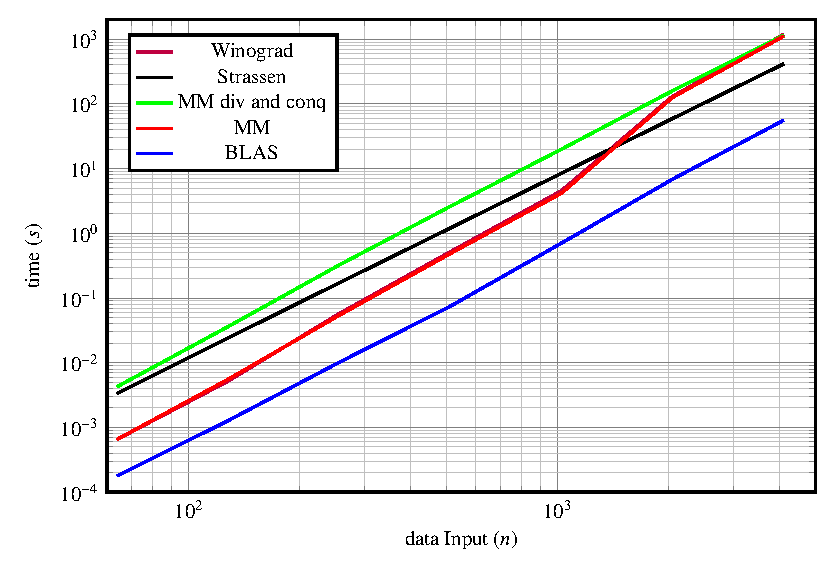
\includegraphics[width=\linewidth]{papers/multiplikation/images/meas_c}
	\caption{Doppelt logarithmisch dargestellte Laufzeiten, der verschieden Algorithmen, in der Programmiersprache \texttt{C}.
	Die Steigung der Messreihe mit Strassens Algorithmus ist deutlich kleiner als deren der anderen Algorithmen.
	Die Messung von Winograd ist beinahe gleich wie die Messung mit der Standardmethode, deshalb ist sie nicht gut sichtbar.}
	\label{multiplikation:fig:c_meas_4096}
\end{figure}


\begin{figure}
	\center
	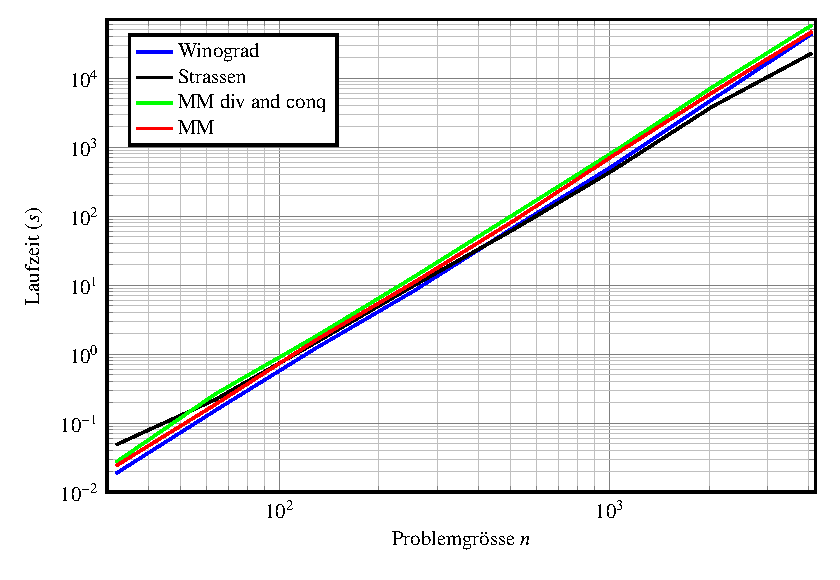
\includegraphics[width=\linewidth]{papers/multiplikation/images/meas_python}
	\caption{Doppelt logarithmisch dargestellte Laufzeiten, der verschieden Algorithmen, in der Skriptsprache \texttt{Python}.
	Die Steigung der Messreihe mit Strassens Algorithmus ist deutlich kleiner als deren der anderen Algorithmen.
}
	\label{multiplikation:fig:python}
\end{figure}

\section{Fazit}
\rhead{Fazit}

Wie man im Abschnitt \ref{multiplikation:section:Implementation} sehen kann, sind die gezeigten Algorithmen trotz der theoretisch geringeren Zeitkomplexitäten den Implementationen der numerischen Bibliotheken klar unterlegen.
Ein optimierter Speicherzugriff hat einen weitaus grösseren Einfluss auf die Laufzeit als die Zeitkomplexität des Algorithmus.

Doch haben Entdeckungen wie jene von Strassen und Winograd ihre Daseinsberechtigung.
Nicht auf jeden Computersystemen können die \textit{BLAS} angewandt werden.
Denke man an sehr kleine Mikrocontroller ohne Floatingpoint Recheneinheiten oder auch an \textit{Field Programmable Gate Arrays (FPGA's)}.
Der Overhead der gezeigten Algorithmen ist in allen Fällen grösser als bei der Standardmethode (z.B. sieben rekursive Aufrufe gegenüber drei \texttt{for}-Schleifen).
Um diesem entgegenzuwirken muss der Laufzeitunterschied zwischen Addition und Multiplikation gross genug sein.
Wenn dies gegeben ist und dazu noch grosse Matritzen multipliziert werden, kann die Verwendung der Algorithmen von Strassen oder Winograd zu einer Senkung der Laufzeit führen.
